\chapter{Metodologías Ágiles}
\label{ch:agil}

\section{Características Generales}
\label{sec:caracteristicas}
La primera vez que el término \emph{ágil} es aplicado al desarrollo del
software es en 2001, gracias a un grupo de expertos en la ingeniería
del software reunidos en Utah. El objetivo del encuentro era
establecer qué principios y valores debería tener un equipo de
desarrollo para poder producir software, de calidad, rápidamente y
pudiendo reaccionar ante los cambios surgidos durante la vida del
proyecto. En resumen, ofrecer una alternativa a los modelos de proceso
de la ingeniería del software tradicional.

Fruto de la reunión fue la creación de la organización, sin ánimo de
lucro, \emph{The Agile Alliance} cuyo propósito es promover el desarrollo
\emph{ágil} de software y ayudar a las empresas a adoptar esta nueva
metodología de trabajo. La filosofía \emph{ágil} se resume en el documento
\emph{Manifiesto Ágil}, ver Figura~\ref{fig:manifiesto}.

\begin{figure}[h]
\hrule\smallskip
\begin{center}
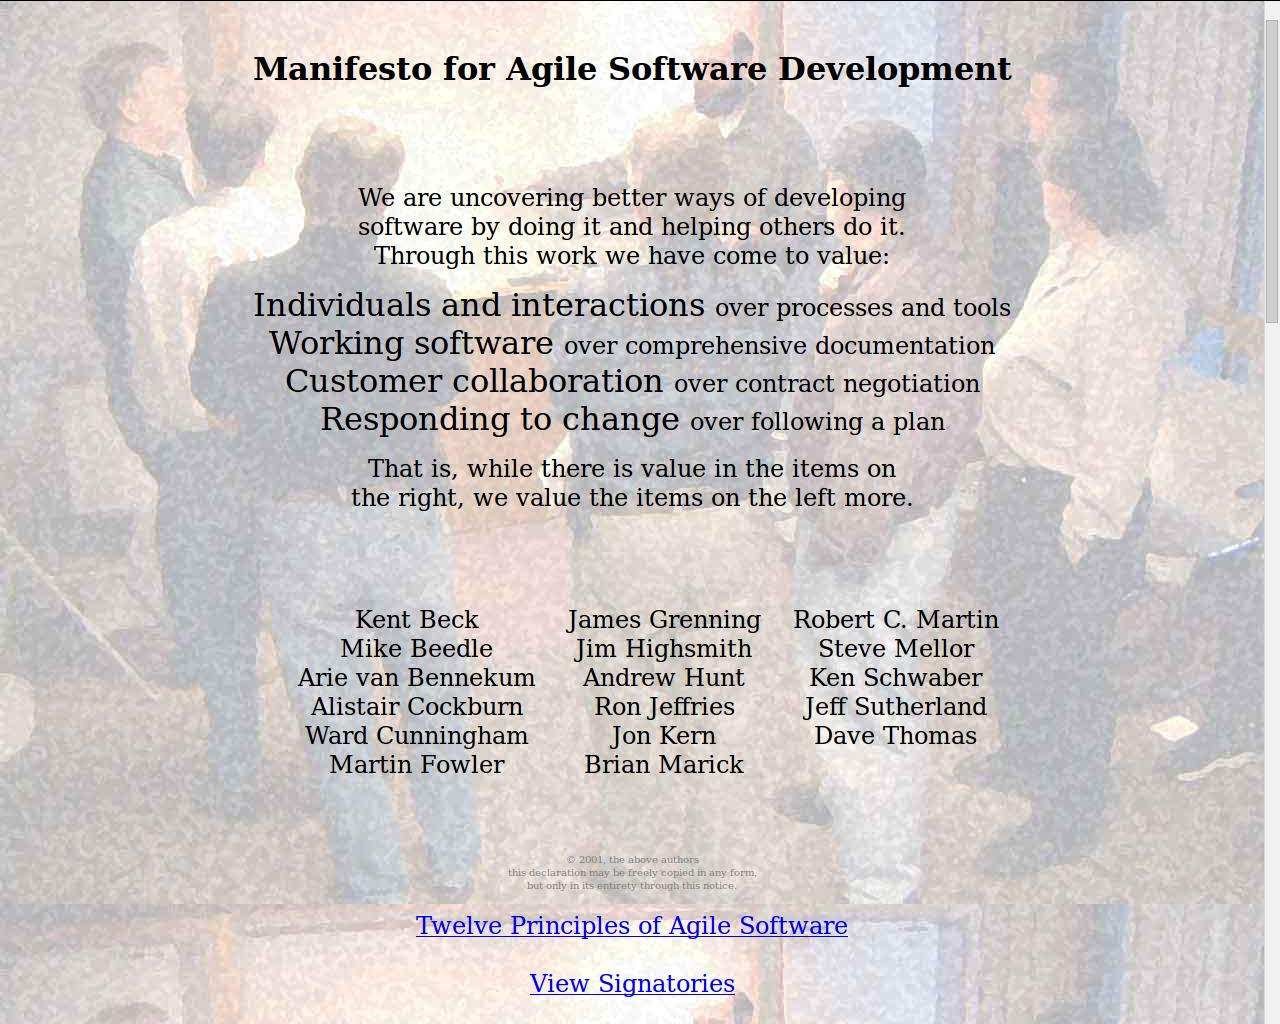
\includegraphics[width=0.7\textwidth]{fig/manifiesto.jpg}
\end{center}
\caption{Manifiesto Ágil, en su web}
\label{fig:manifiesto}
\hrule
\end{figure}

El manifiesto expresa que, aunque aprecian y tienen en cuenta los
elementos básicos del desarrollo del software tradicional
(documentación, procesos, herramientas, plan de trabajo,..) prefieren
sobreponer otros elementos, otros valores:
\begin{itemize}
\item Individuos e interacciones sobre las herramientas y los
  procesos.
\item Software funcional sobre documentación extensa.
\item Colaborar con el cliente frente a una negociación contractual.
\item Posibilidad de respuesta al cambio frente a seguir un plan
  cerrado.
\end{itemize}

Estos valores producen los doce principios que encontramos en el
manifiesto, ver Figura~\ref{fig:principios}

\begin{figure}[h]
\hrule\smallskip
\begin{center}
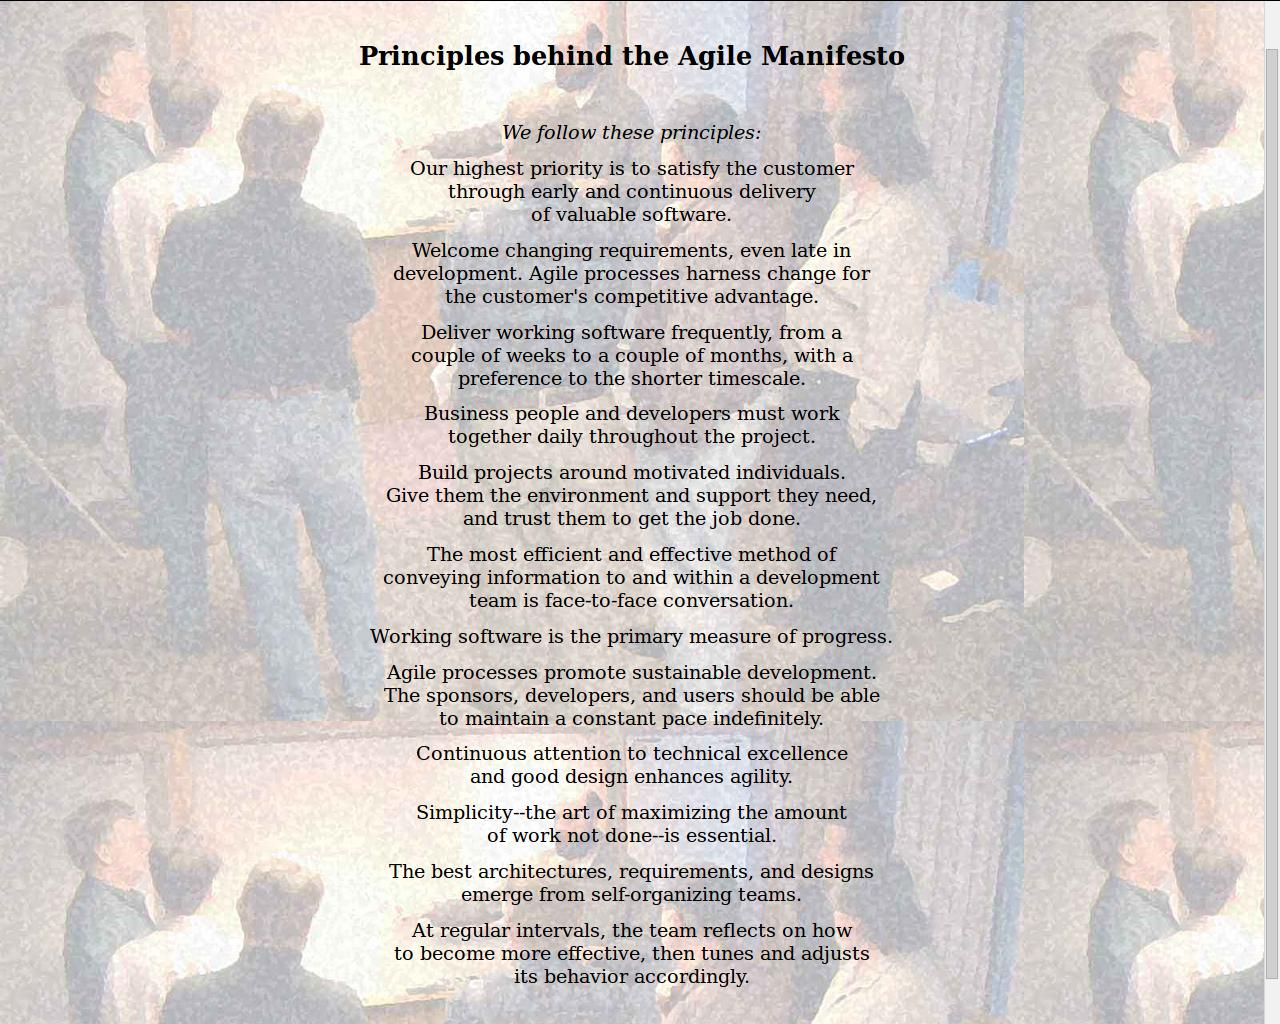
\includegraphics[width=0.7\textwidth]{fig/principios.jpg}
\end{center}
\caption{Principios del Manifiesto Ágil, en su web}
\label{fig:principios}
\hrule
\end{figure}

Estos principios marcan la diferencia entre los procesos tradicionales
y los considerados ágil. Los dos principios iniciales son genéricos a
todo el proceso, se consideran un resumen del estilo ágil.


\section{Programación Extrema}
\label{sec:xp}

La programación extrema (XP) es una de estas metodologías ágil que se
basa en los cuatro valores descritos en el apartado anterior y sigue
sus doce principios. En concreto esta metodología se diseña para
proyectos con requisitos muy imprecisos y cambiantes donde la relación
con el cliente y una buena comunicación en el equipo son esenciales.

El apellido \lst{extrema} se lo da Kent Beck, uno de los firmantes del
manifiesto ágil, porque coge los principios y los lleva al extremo en
la aplicación. Se asume que el proyecto va a tener muchos cambios y se
quiere reducir el coste de aplicarlos. Algunas de las características
son:
\begin{itemize}
\item Comunicación entre cliente y programadores de manera directa
  aunque supervisada. Siempre que se habla de la herramienta a
  desarrollar habrá al menos un experto miembro del equipo de
  desarrollo presente.
\item Se produce rápido por medio de entregas pequeñas. Se pone como
  máximo 3 meses para realizar una entrega. Aunque se recomienda no
  llegar a tanto.
\item La herramienta se describe mediante metáforas, ayudando a
  cliente y desarrolladores a hablar de lo mismo sin utilizar
  tecnicismos.
\item Se diseña siempre pensando en la simplicidad, se debe
  implementar la solución más sencilla que funcione.
\item Cada modificación realizada en el desarrollo debe superar una
  batería de pruebas unitarias establecidas con el cliente.
\item Trabajar en parejas es un requisito de modo que se reducen
  errores, se mejora el diseño, etc.
\item Se establece un máximo en el número de horas semanales, nadie
  podrá trabajar más de 40 horas a la semana.
\item El cliente debe tener disponibilidad constante para el equipo.
\item Programación mediante estándares, de modo que todo programador
  que coja el código sepa que ha hecho un programador anterior.
\end{itemize}
Estas prácticas junto con otras conforman la manera de trabajar
mediante una metodología XP. En Figura~\ref{fig:xp} podemos ver la
relación entre estas prácticas de modo que si tienen una flecha
significa que se refuerzan mutuamente.


\begin{figure}[h]
\hrule\smallskip
\begin{center}
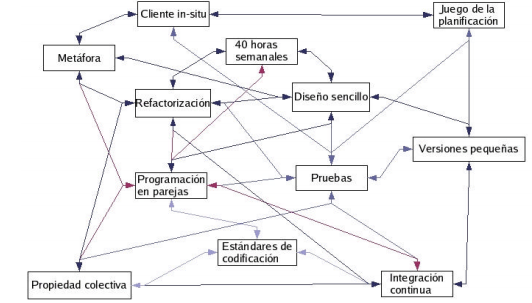
\includegraphics[width=0.9\textwidth]{fig/xp.png}
\end{center}
\caption{Relación de las características de XP}
\label{fig:xp}
\hrule
\end{figure}


Para llevar a cabo estas prácticas se utiliza una técnica conocida
como \emph{Historias de Usuario} donde se especifican los requisitos
mediante tarjetas de papel en las cuales el cliente describe
brevemente lo que un usuario debe poder hacer con la herramienta.

Kent Beck además define diferentes roles y dice que cada participante
en el proyecto debe tener uno de ellos:
\begin{itemize}
\item Programador
\item Cliente
\item Tester
\item Tracker
\item Entrenador
\item Consultor
\item Gestor
\end{itemize}

Las etapas del desarrollo quedan establecidas en 4, de manera cíclica:
\begin{enumerate}
\item El cliente define historias de usuario y su valor de negocio.
\item El programador estima el esfuerzo necesario para llevarlas a
  cabo.
\item El cliente decide qué se debe construir y sus prioridades,
  teniendo en cuenta las posibles restricciones de tiempo.
\item El programador implementa lo acordado.
\item Se vuelve al paso 1 hasta terminar el proyecto. Del 1 al 4 no
  deben pasar más de 3 meses.
\end{enumerate}

\section{Scrum}
\label{sec:scrum}

Scrum es una metodología ágil que se basa en la experiencia del equipo
y el conocimiento de los integrantes para realizar un desarrollo
fiable, de calidad y con producción incremental. Por eso se puede
decir que se caracteriza por:
\begin{itemize}
\item Adoptar una estrategia de desarrollo incremental, en lugar de la
  planificación y ejecución completa del producto.
\item Basar la calidad del resultado en el conocimiento tácito de las
  personas del equipo auto organizado.
\item Solapar las diferentes fase de desarrollo, en lugar de
  realizarlas de forma secuencial como ocurriría en otras metodologías
  más tradicionales.
\end{itemize}
Para llevar a cabo esta metodología se definen tres roles y divide el
tiempo en \lst{sprints}. Estos \lst{sprints} son la unidad básica de
medida y planificación. Se puede establecer la duración de un
\lst{sprint} en 10 días, aunque la duración puede variar en función de
la experiencia del equipo de desarrollo y de las tareas a
realizar. Suponiendo un \lst{sprint} de 10 días se sigue la siguiente
planificación:
\begin{itemize}
\item Día 1: Reunión de planificación del Sprint. Tiene una duración
  máxima de una hora. Se define que se desea hacer durante ese
  sprint. Se debe generar un acta o log con lo acordado.
\item Día 2-9: Reunión de Sprint. Tiene una duración máxima de 15
  minutos. Se realiza todos los días del sprint. No se realiza acta de
  la reunión. El ScrumMaster realiza a cada miembro del equipo las
  siguientes preguntas:
  \begin{itemize}
  \item ¿Qué hiciste ayer?
  \item ¿Qué harás para mañana?
  \item ¿Te ha surgido algún problema?
  \end{itemize}
\item Día 10: Reunión de Revisión del Sprint: Tiene una duración
  máxima de una hora. Se revisa el trabajo realizado y los objetivos
  alcanzados. Se puede mostrar demos del trabajo finalizado, pero
  nunca de partes parciales. Se genera un acta detallando los
  objetivos no alcanzados.  
\end{itemize}
Para garantizar la calidad de esta metodología basada en la calidad
del equipo de desarrollo se deben definir claramente unos roles que
garanticen el buen funcionamiento de la misma.
\begin{itemize}
\item \lst{Product Owner}: representa la voz del cliente. Se asegura
  de que se realicen las tareas adecuadamente desde una perspectiva de
  negocio.
\item \lst{Scrum Master (facilitador)}: trata de eliminar todos los
  obstáculos que impiden que el equipo alcance los objetivos del
  Sprint actual. No es el líder del equipo, el equipo es
  auto-organizado. El ScrumMaster asegura que el equipo no se
  distraiga del objetivo y cumpla las reglas de la metodología Scrum.
\item \lst{Desarrollador}: Realiza el producto con su equipo.
\end{itemize}
